% CNN %

%\subsection{CNN}\label{sub:cnn}

We set up a convolutional neural network with the preprocessed oct images as input.
The main idea is, that force acts continuously on the tissue and therefore its value depends on the past.
By considering several A-scans for force estimation at one timestamp, outliers are weakened and local connectivity between actual
measurement data and past data is created.

    \textit{Architecture} The image size of the oct is defined by the number of A-scans, whereby one A-scan contains data of 101 pixels.
To obtain a desired input image size $H$x$W$ for the model, the whole B-scan $H$x$W'$ is splitted by windowing it with a stride of 1.
Thus, a dimension of $D=W'-W-1$ of the input image arises.
The architecture of our CNN is adapted to ~paper gel force estimation~.
Due to the small amount of data, we use one convolutional layer followed by a rectified linear units layer and one 2x2 max pooling layer with a stride of two. 
The convolutional layer has 32 filter with size of 3x6 and a stride of one.

\begin{figure}
    \centering
    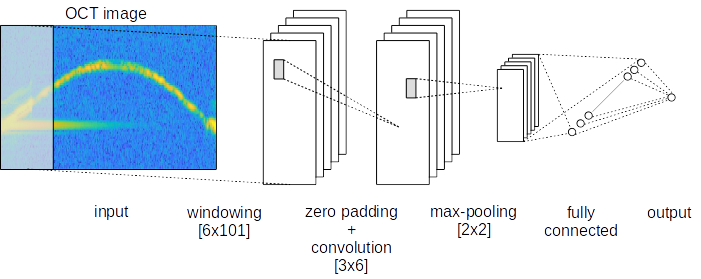
\includegraphics[width=0.9\textwidth]{cnn.png}
    \caption{Architecture of the CNN}
    \label{fig:cnn_archi}
\end{figure}

